\chapter{Caso de uso: Sistema de Registro de Asistencia y Monitoreo de Aulas}\label{chap:7}

En este capítulo se pone a prueba LoRaLAN con la aplicación que motivó el trabajo, el sistema de registro de asistencia del profesorado y monitorización de aulas implementado sobre la red Wi-Fi del edificio, que se migra a una red LoRaLAN. A continuación, se describen la arquitectura extremo a extremo, la capa de aplicación diseñada sobre LoRaLAN, encargada de comunicar los nodos con el servidor, y el recorrido de un fichaje. Además se muestra el diseño llevado a cabo para fabricar una PCB para el prototipo y posteriormente se detalla el servidor, la base de datos y, finalmente, se exponen las pruebas realizadas y se expone el diseño y empleo de un monitor de red a partir de un Cardputer M5 con un módulo SX1262.

\section{Sistema de partida y requisitos}

El sistema, desarrollado en el Centro Universitario de Mérida, como ya se ha comentado anteriormente, consta de un dispositivo por aula basado en ESP32, con un lector NFC para la tarjeta del profesor, sensores ambientales y de presencia, dos relés e indicadores. La aplicación se conecta con un servidor desarrollado con FastAPI en Python e implementa persistencia conectándose a una base de datos relacional con MySQL. El servidor decide si los registros de asistencias son válidos verificando la tarjeta con el horario del aula. Además el sistema ofrece paneles web para que los profesores puedan consultar sus horarios lectivos y el recuento de clases impartidas al mes. A los conserjes se les facilita un panel que permite consultar el estado de las aulas y la información relativa a sus sensores. A los administradores se les facilita un panel para administrar los nodos LoRaLAN. El dispositivo y el servidor se comunicaban a través de la red Wi-Fi del edificio, por la que el dispositivo enviaba los fichajes por HTTP y mantenía una conexión WebSocket permanente para la telemetría y las órdenes. 

La especificación de requisitos completa se recoge en el Capítulo~\ref{chap:3}. Los casos de uso que atraviesan la red de radio son fichar, supervisar un aula, accionar un relé y reiniciar un dispositivo.

La correspondencia con las clases de tráfico del apartado~\ref{sec:escenario} es directa, ya que el fichaje es el evento, la telemetría es el tráfico periódico y los relés son las órdenes.

\section{Arquitectura de extremo a extremo}

En la Figura~\ref{fig:arquitectura} se muestra la arquitectura del sistema tras la migración, junto con los tres flujos que la recorren: el fichaje, la monitorización y el control.

\begin{figure}[H]
\centering
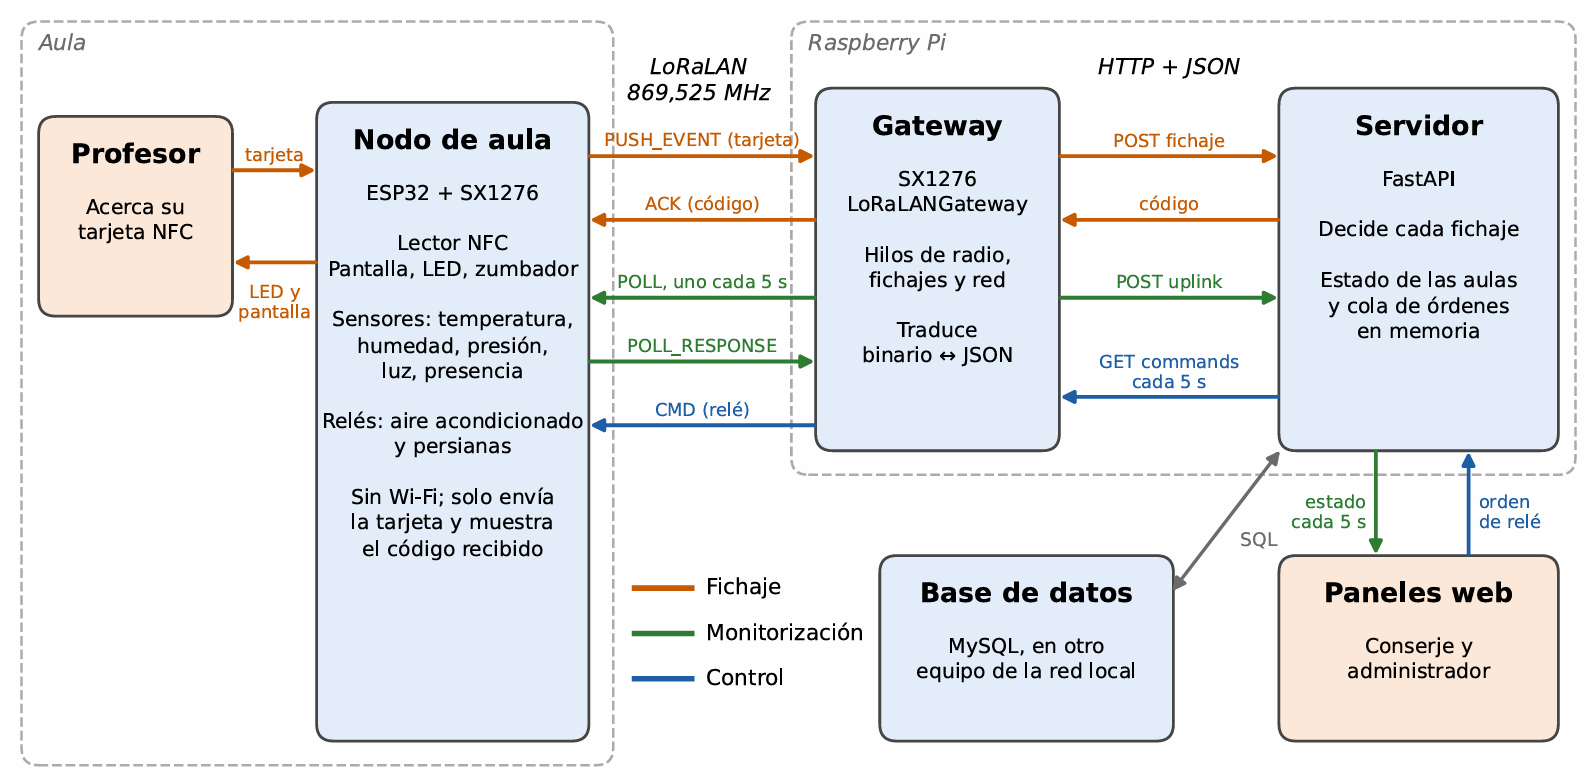
\includegraphics[width=\textwidth]{imagenes/esquema de fichaje.png}
\caption{\label{fig:arquitectura} Arquitectura del sistema de registro de asistencia y monitoreo de nodos sobre LoRaLAN.}
\end{figure}

El nodo de aula se limita a enviar el identificador de la tarjeta leída y la telemetría, y a mostrar el código de resultado recibido. El gateway, ejecutado en una Raspberry Pi, es el único punto de contacto entre las redes de radio e IP y traduce los mensajes binarios de los nodos a peticiones HTTP con cuerpo JSON, y viceversa. El servidor implementa la lógica de negocio y la gestión de la base de datos, pero se comunica exclusivamente con el gateway, mientras que los paneles web consultan periódicamente su estado. En el prototipo, el gateway y el servidor se ejecutan en la misma Raspberry Pi, mientras que la base de datos se puede ejecutar en el mismo equipo o en otra máquina.

La migración elimina todas las conexiones WebSocket y sustituye la comunicación permanente por consultas periódicas del gateway al servidor. Esto se realiza para centralizar el control de las transmisiones en el gateway. De este modo, el servidor registra las órdenes pendientes y el gateway las consulta y transmite cuando considera oportuno o cuando su presupuesto de ciclo de trabajo lo permite.

La lógica de negocio sobre los fichajes sigue correspondiendo al servidor, que conoce la existencia de las tarjetas, los horarios de clase y los profesores asignados a cada asignatura. Esto simplifica el nodo y evita distribuir información de horarios por la red de radio, aunque exige que la respuesta llegue al nodo dentro del plazo de un intercambio. Este requisito motivó la confirmación con carga útil del protocolo (apartado~\ref{sec:ackdiferido}).

\section{Capa de aplicación sobre LoRaLAN}\label{sec:appprotocol}

Dado que LoRaLAN transporta cargas opacas, su significado lo define una capa de aplicación propia que se especifica en un único fichero de cabecera, \texttt{AppProtocol.h}, compartido por el firmware del nodo y el gateway, de modo que ambos extremos compilan la misma definición. El primer byte de cada mensaje identifica su tipo y los valores de varios bytes viajan con el byte más significativo en primer lugar (\textit{big-endian}), como se muestra en la Tabla~\ref{tab:appmsg}. La idea es implementar una capa de aplicación sencilla que sea capaz de transportar la mayor cantidad de información en el menor número de bytes posible.

\begin{table}[H]
\centering
\small
\caption{\label{tab:appmsg} Mensajes de la capa de aplicación.}
\begin{tabular}{|c|l|c|p{4.6cm}|p{3cm}|}
\hline
\textbf{Tipo} & \textbf{Mensaje} & \textbf{Bytes} & \textbf{Contenido} & \textbf{Transporte} \\
\hline
\texttt{0x01} & FICHAJE & 5--11 & Identificador de la tarjeta (4 a 10 bytes) & PUSH\_EVENT con confirmación diferida \\
\hline
\texttt{0x02} & SENSORES & 10 & Temperatura, humedad, presión, iluminación y presencia & POLL\_RESPONSE \\
\hline
\texttt{0x03} & ESTADO\_RELES & 2 & Un bit por relé & POLL\_RESPONSE \\
\hline
\texttt{0x10} & RELE & 3 & Número de relé y estado deseado & CMD \\
\hline
\texttt{0x11} & RESET & 1 & --- & CMD \\
\hline
\end{tabular}
\end{table}

Las magnitudes físicas se codifican como enteros de 16~bits en coma fija, de modo que una lectura completa ocupa 10~bytes cuando un JSON equivalente ocuparía varias veces más, diferencia que en la transmisión por radio afecta directamente al tiempo en el aire. Un sensor sin lectura válida se codifica con un valor reservado que el gateway traduce a nulo, y la orden RELE transporta el estado deseado y no una conmutación, por lo que repetirla no tiene efecto adicional.

La respuesta a un registro es un único byte que viaja dentro del ACK y que puede tomar los valores de la Tabla~\ref{tab:codigos}. Los códigos 1 a 3 son \textbf{definitivos}, puesto que reintentar no cambiaría el resultado, mientras que el 4 es \textbf{temporal}, y un código que el nodo no reconozca se trata también como temporal, ya que ante la duda es preferible reintentar que dar por perdido un fichaje.

\begin{table}[H]
\centering
\small
\caption{\label{tab:codigos} Códigos de resultado de un fichaje.}
\begin{tabular}{|c|l|p{4.3cm}|p{5cm}|}
\hline
\textbf{Código} & \textbf{Nombre} & \textbf{Significado} & \textbf{Reacción del nodo} \\
\hline
0 & OK & Asistencia registrada & LED verde. \\
\hline
1 & SIN\_CLASE & No hay clase en esa aula a esa hora & LED amarillo. No reintenta. \\
\hline
2 & DENEGADO & La clase es de otro profesor & LED rojo. No reintenta. \\
\hline
3 & DESCONOCIDO & Tarjeta no registrada o nodo sin aula & LED rojo. No reintenta. \\
\hline
4 & REINTENTAR & El servidor no ha podido responder & LED amarillo intermitente. Guarda el fichaje y lo reenvía. \\
\hline
\end{tabular}
\end{table}

\section{Flujos de extremo a extremo}

\subsection{Fichaje}

A continuación se resume el recorrido de un registro de asistencia por parte de un profesor:

\begin{enumerate}[label=\protect\circled{\arabic*}, leftmargin=*, itemsep=0.2em]

    \item El usuario se identifica con su tarjeta en el Nodo~2. % REVISAR
    \item El nodo envía una trama LoRaLAN de datos al gateway y espera el ACK.
    \item El gateway valida la trama y reenvía la carga útil al servidor FastAPI.
    \item El servidor valida el fichaje y lo registra en la base de datos.
    \item El servidor devuelve el resultado al gateway.
    \item El gateway transmite por LoRa una trama ACK al nodo.
    \item El nodo comprueba el número de secuencia y confirma el fichaje al
          usuario (pantalla y LED verde). Si el ACK no llega, retransmite.
    \item El panel web consulta el servidor y muestra que en esa aula hay una clase en curso.
\end{enumerate}


\begin{figure}[H]
\centering
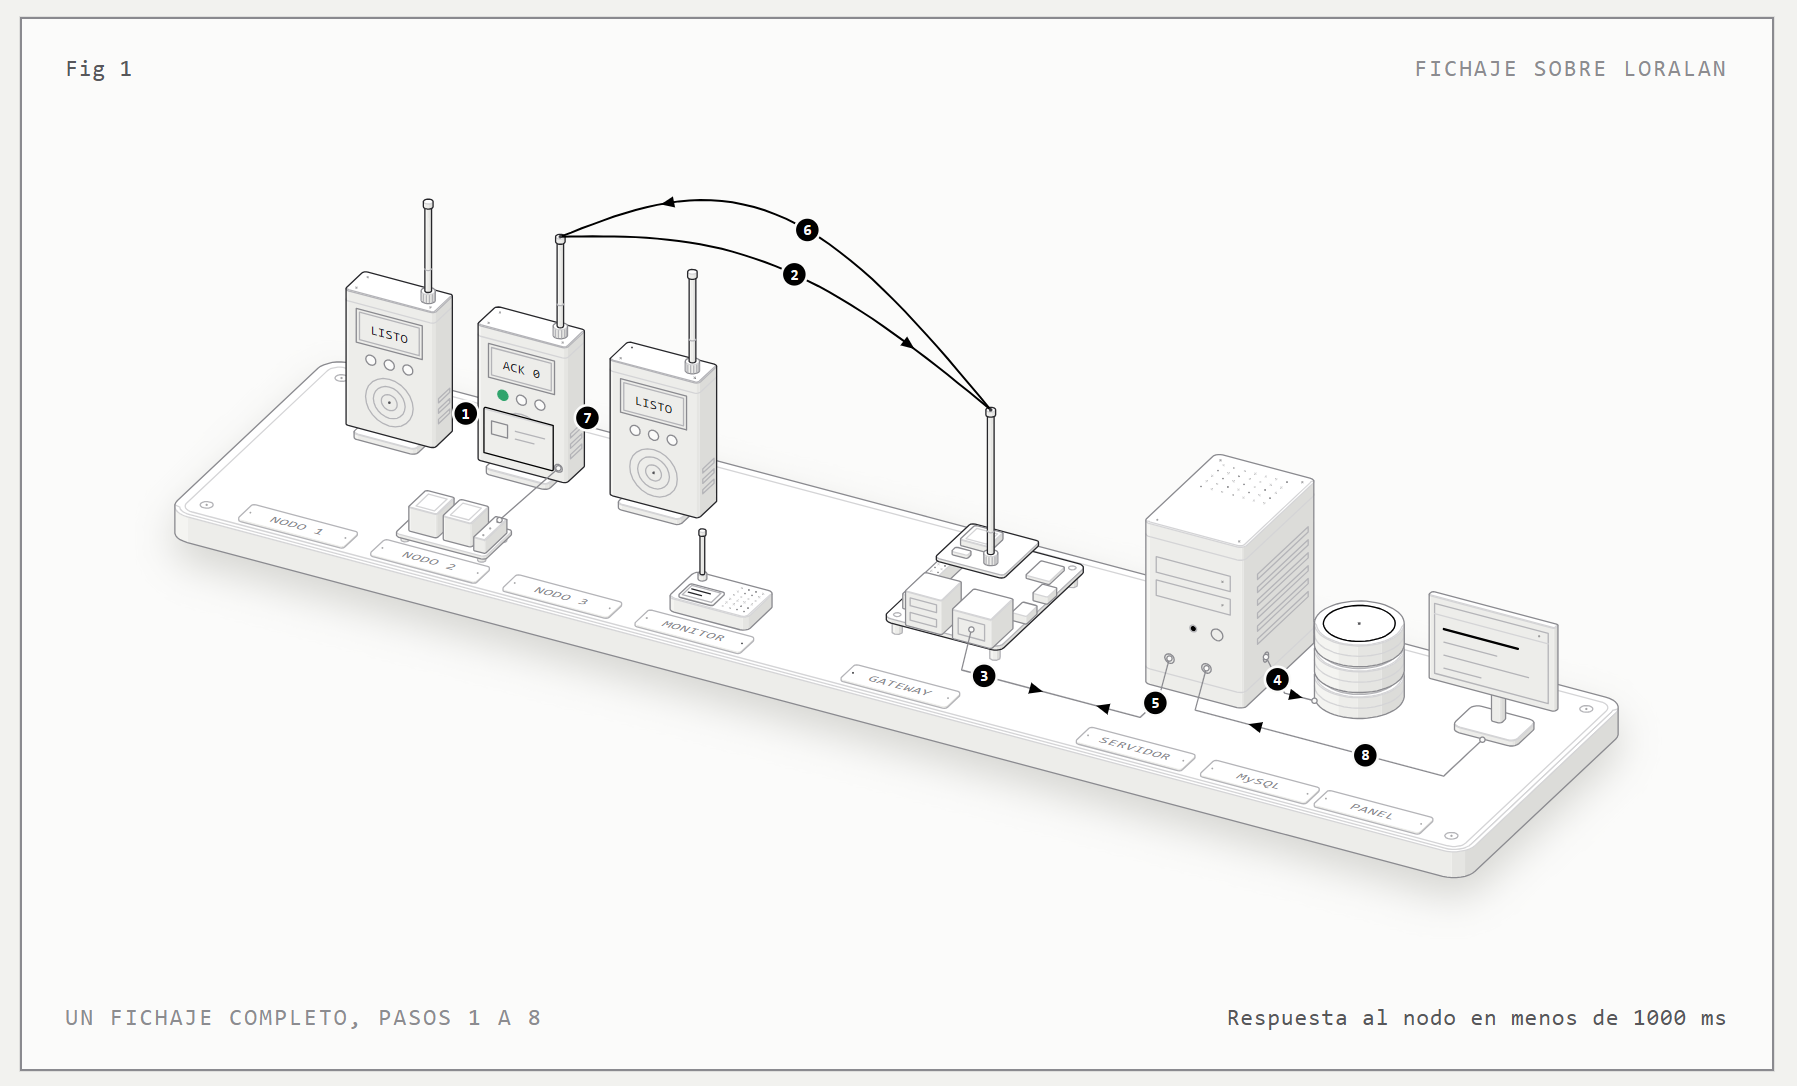
\includegraphics[width=0.92\textwidth]{imagenes/fichajeSatisfecho.png}
\caption{\label{fig:fichaje} Secuencia de un fichaje aceptado.}
\end{figure}

Con SF7, el intercambio de radio consta de dos tramas: 51,5~ms de ida
(identificadores de 4 a 7~bytes) y 41,2~ms de vuelta; el resto depende del
servidor. Para que el nodo reciba siempre una respuesta, se encadenan tres
plazos: la petición HTTP se abandona a los 800~ms, el gateway responde
REINTENTAR a los 1000~ms (descartando respuestas posteriores) y el nodo no
retransmite hasta los 1200~ms. Así, ante un servidor lento o caído, el nodo
obtiene una respuesta explícita en torno a un segundo en lugar de agotar sus
reintentos y ocupar el canal. Los casos de error se resuelven así:

\begin{itemize}
    \item \textbf{Servidor sin respuesta}: el nodo guarda el fichaje en una
    cola en memoria (hasta ocho elementos) y lo reenvía cada 30~s hasta
    obtener un código definitivo, sin que el profesor repita el fichaje.
    \item \textbf{ACK perdido}: el gateway reconoce el número de secuencia de
    la retransmisión y reenvía el mismo ACK sin consultar al servidor.
    \item \textbf{Respuesta tardía del servidor}: el fichaje reenviado ya está
    registrado; el servidor detecta la asistencia existente (profesor, clase
    y aula) y responde OK sin duplicarla.
    \item \textbf{Reinicio del nodo}: los fichajes en cola se pierden al
    residir en memoria volátil, limitación asumida en el prototipo.
\end{itemize}

La fiabilidad de extremo a extremo no depende de una sola capa: LoRaLAN evita
los duplicados de radio y la aplicación, los de aplicación.

\subsection{Telemetría y órdenes}

La telemetría se apoya en el sondeo. Cuando el gateway sondea a un nodo, este responde con el estado de los relés si ha cambiado. Una orden de relé recorre el camino contrario: el panel la envía al servidor, que la encola; el gateway la recoge en su siguiente consulta y la transmite como paquete de tipo CMD; y el nodo actúa sobre la salida e informa de su nuevo estado en el sondeo siguiente. Por tanto, el panel no muestra lo que se ha ordenado, sino lo que el nodo confirma que ha hecho.

\section{Backend FastAPI}

El servidor se organiza en tres capas: los \textit{routers} declaran las operaciones HTTP y validan sus datos con modelos de Pydantic, los servicios contienen la lógica de negocio y los repositorios encapsulan las consultas a la base de datos. Las operaciones se resumen en la Tabla~\ref{tab:endpoints}.

\begin{table}[H]
\centering
\small
\caption{\label{tab:endpoints} Operaciones del servidor.}
\begin{tabular}{|l|l|l|p{6.2cm}|}
\hline
\textbf{Método} & \textbf{Ruta} & \textbf{Rol} & \textbf{Función} \\
\hline
POST & \texttt{/auth/device} & --- & Entrega un \textit{token} al gateway a cambio de su nombre y su clave. \\
\hline
POST & \texttt{/auth/login} & --- & Valida el correo y la contraseña, entrega el \textit{token} del usuario en una \textit{cookie} \texttt{HttpOnly} y lo redirige al panel de su rol. \\
\hline
GET & \texttt{/logout} & --- & Borra la \textit{cookie} de sesión. \\
\hline
POST & \texttt{/gateway/fichaje} & Gateway & Registra un fichaje y devuelve el código de resultado. \\
\hline
POST & \texttt{/gateway/uplink} & Gateway & Recibe sensores, estado de relés y altas/bajas de nodos. \\
\hline
GET & \texttt{/gateway/commands} & Gateway & Entrega y vacía la cola de órdenes del gateway. \\
\hline
POST & \texttt{/gateway/status} & Gateway & Recibe nodos, tráfico, descartes y ciclo de trabajo. \\
\hline
GET & \texttt{/panel/estado} & Conserje, admin. & Estado de las aulas y, para el administrador, de la radio y los gateways. \\
\hline
POST & \texttt{/panel/rele} & Conserje, admin. & Encola una orden de relé. \\
\hline
POST & \texttt{/panel/reset} & Admin. & Encola un reinicio del nodo. \\
\hline
POST & \texttt{/panel/aula} & Admin. & Asigna un aula a un nodo. \\
\hline
\end{tabular}
\end{table}

La operación de fichaje responde siempre con éxito HTTP y devuelve el resultado en el campo \texttt{code}, puesto que el gateway necesita un byte para el ACK y no un estado que interpretar. Para decidirlo, el servidor busca al profesor por la tarjeta y el aula asignada al nodo, y responde DESCONOCIDO si falta alguno; busca después la clase de esa aula en ese momento, primero en la base de datos y, si no la encuentra, consulta el servicio de reservas de la universidad. Responde SIN\_CLASE si no la hay o DENEGADO si es de otro profesor; y, por último, registra la asistencia salvo que ya exista una de ese profesor en esa clase y esa aula, respondiendo OK en ambos casos. Cualquier error interno se traduce en REINTENTAR y nunca en un código definitivo, que haría que el nodo descartase un fichaje legítimo.

En cuanto a la autenticación, el servidor emite \textit{tokens} JWT para dos tipos de cliente. Las personas inician sesión con su correo y una contraseña almacenada como \textit{hash} bcrypt, y su \textit{token} viaja en una \textit{cookie} \texttt{HttpOnly} que se comprueba en cada operación según el rol, mientras que el gateway presenta un \textit{token} de dispositivo que renueva cuando caduca. El servidor comprueba además que el gateway nombrado en cada petición coincide con el del \textit{token}, impide que un nodo del sistema antiguo actúe como gateway y limita los intentos de autenticación por dirección IP.

El último estado de cada aula y la cola de órdenes se mantienen en memoria, y un nodo se considera conectado si el gateway ha subido algo suyo en los últimos 120~segundos. Un reinicio del servidor pierde, por tanto, las órdenes no recogidas, aunque el estado se reconstruye con los siguientes sondeos. Los paneles consultan ese estado cada 5~segundos: el conserje ve las aulas y acciona sus relés, y el administrador ve además los datos de radio de cada nodo y el consumo de ciclo de trabajo de los gateways.

\section{Base de datos}

La base de datos consta de las cinco tablas que se muestran en el diagrama entidad-relación de la Figura~\ref{fig:er}.

\begin{figure}[H]
\centering
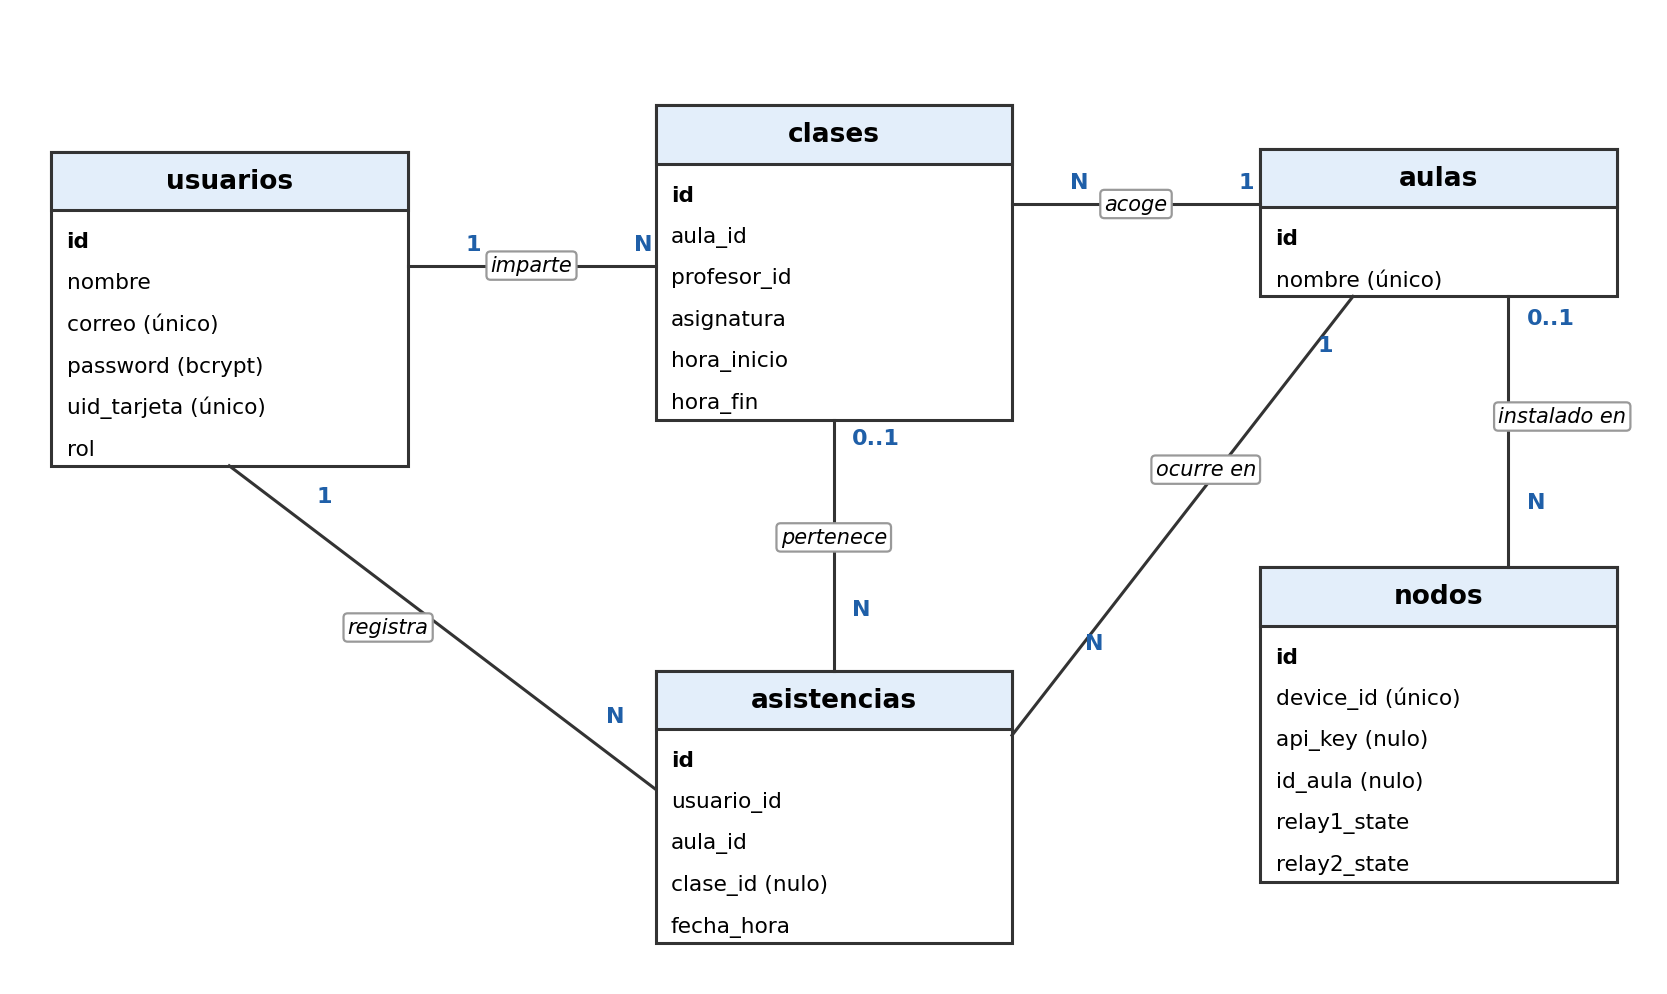
\includegraphics[width=0.9\textwidth]{imagenes/er_fichaje.png}
\caption{\label{fig:er} Diagrama entidad-relación de la base de datos del sistema de la aplicación.}
\end{figure}

La tabla de usuarios recoge profesores, conserjes y administradores. Aulas identifica las aulas por un nombre único. Clases relaciona profesores, aulas y franjas horarias. Asistencias registra los fichajes aceptados y nodos almacena los dispositivos LoRaLAN y gateways, junto con su identificación, aula asignada y estado de los relés.
Las claves ajenas mantienen la integridad referencial, con dos excepciones deliberadas: al eliminar un aula, sus nodos quedan sin asignación, y al eliminar una clase se conservan las asistencias asociadas. Los nodos se registran automáticamente al recibir su primer paquete y, hasta que el administrador les asigna un aula, sus fichajes reciben el código DESCONOCIDO.


\section{Diseño de la PCB del nodo}\label{sec:pcb}

Las pruebas descritas hasta ahora se realizaron con placas de desarrollo conectadas mediante cableado utilizando una protoboard, una solución adecuada para validar el funcionamiento, pero poco robusta y difícil de replicar en un despliegue real. Además, trabajar sobre una protoboard implica trabajar, habitualmente, con cables que no hacen bien contacto y problemas de conexión que a menudo se solventan asegurando que los cables hacen contacto en sus pines.


Por este motivo, se ha diseñado una placa de circuito impreso (PCB) específica para el nodo LoRaLAN en esta aplicación, que integra en un único soporte las conexiones de todos los componentes.

El diseño se ha realizado con EasyEDA, una herramienta de diseño electrónico que integra en un mismo entorno la captura del esquemático, el diseño de la placa y la generación de los ficheros de fabricación. Además, su biblioteca de componentes hechos por la comunidad permite utilizar casi cualquier componente y cualquier configuración que pueda existir de dicho componente, lo que reduce los errores al pasar del esquemático a la placa y facilita su fabricación por un proveedor externo.

El esquemático, recogido en la Figura~\ref{fig:pcb1}, es el primer paso para generar una PCB. En él se agregan todos los componentes y se realiza el cableado de todos los elementos.

\begin{figure}[H]
\centering
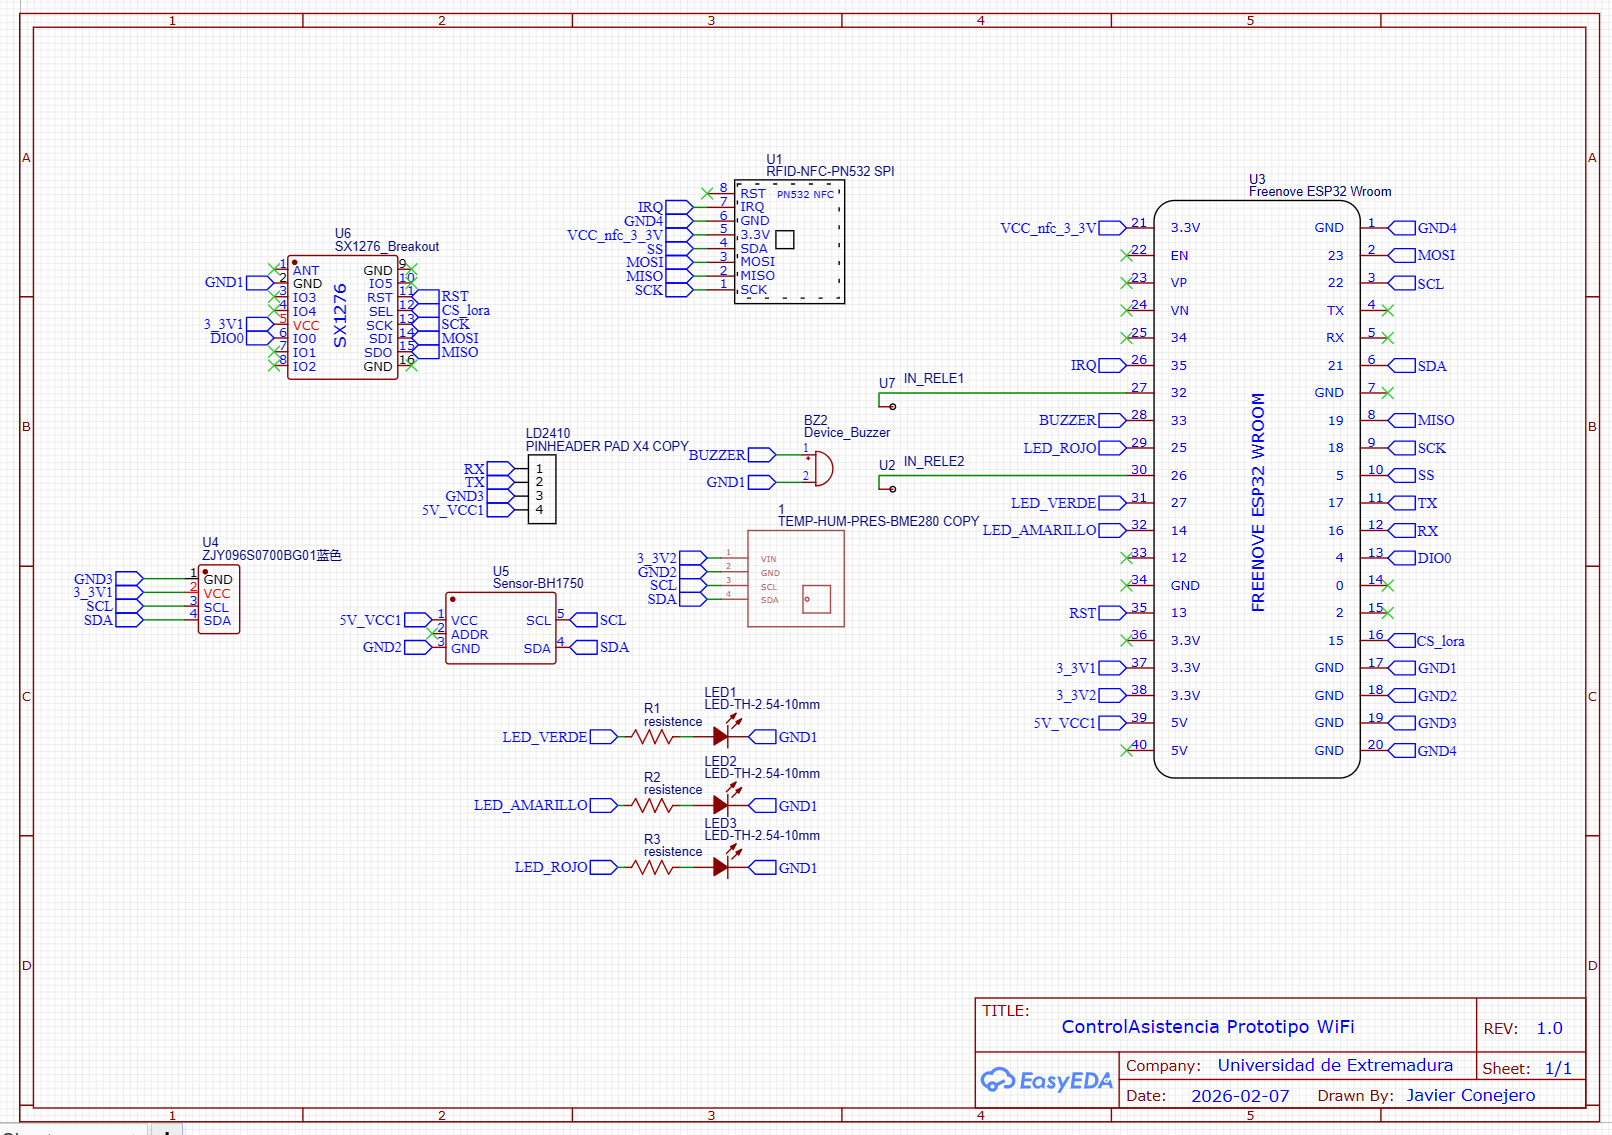
\includegraphics[width=0.9\textwidth]{imagenes/pcb-esquematico.png}
\caption{\label{fig:pcb1} Diagrama de cableado del prototipo de Registro de asistencia.}
\end{figure}

Posteriormente se validan las conexiones del esquemático mediante la comprobación de reglas eléctricas (ERC) y se revisan los \textit{warnings} que aparecen, antes de generar la propia PCB. A continuación se pulsa la opción " Convertir a PCB".

\begin{figure}[H]
\centering
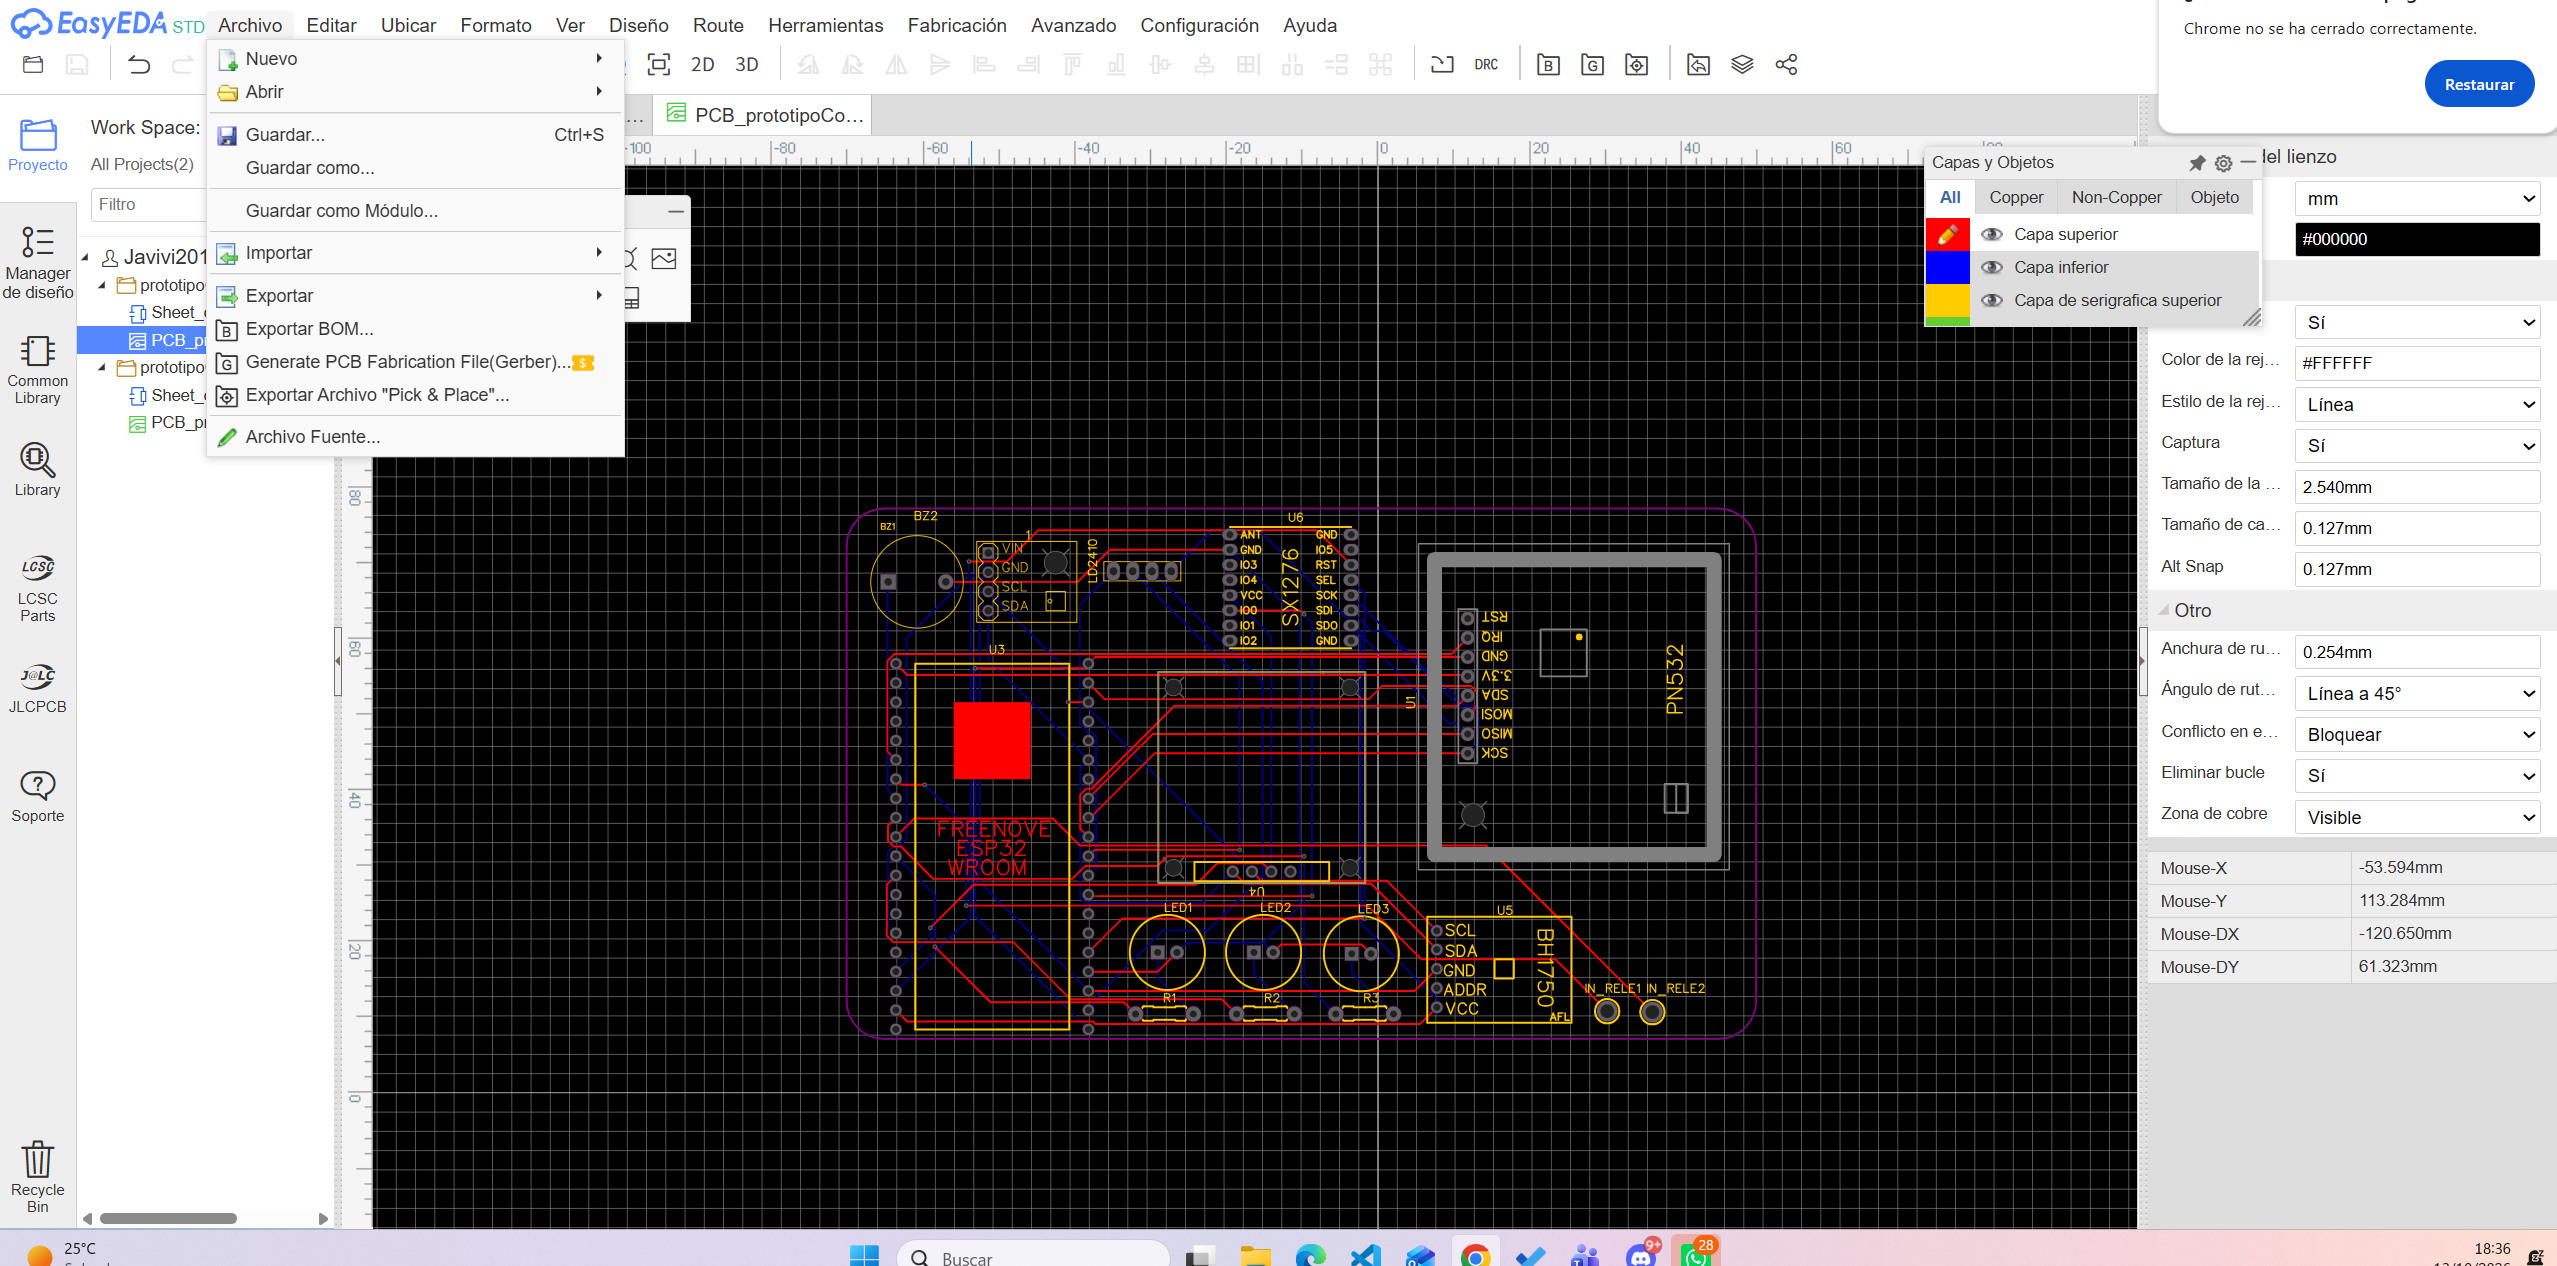
\includegraphics[width=0.9\textwidth]{imagenes/pcb-esquematico2.png}
\caption{\label{fig:pcb2} Previsualización de la PCB de Registro de asistencia.}
\end{figure}

Tal y como se muestra en la Figura~\ref{fig:pcb2}, en esta pantalla se determina cuáles son las dimensiones de la PCB y se posicionan los componentes como se desee. En este caso, se han posicionado todos los elementos intentando minimizar la dimensión de la PCB.

Posteriormente, se utiliza la herramienta auto-ruteo que se encarga de posicionar las pistas sobre las capas de la placa, de manera que no se crucen las pistas entre sí. Además, se tuvo en cuenta que el PN532 debe estar lo más aislado posible, para que no genere interferencias electromagnéticas, dando lugar a errores de lectura.

Por otro lado, el transceptor y la antena se sitúan en un extremo de la placa de forma que la antena sobresalga lo máximo posible para limitar las pérdidas y las interferencias. Por último, se agrega un plano de masa para proporcionar una referencia de 0 V sólida, ofrecer un camino de retorno de corriente de baja impedancia y reducir las interferencias electromagnéticas.


Finalmente, a partir del diseño se mandó fabricar la placa a través de JLCPCB, el fabricante asociado a EasyEDA. En la Figura~\ref{fig:pcb3} se muestra la apariencia final de la PCB.

\begin{figure}[H]
\centering
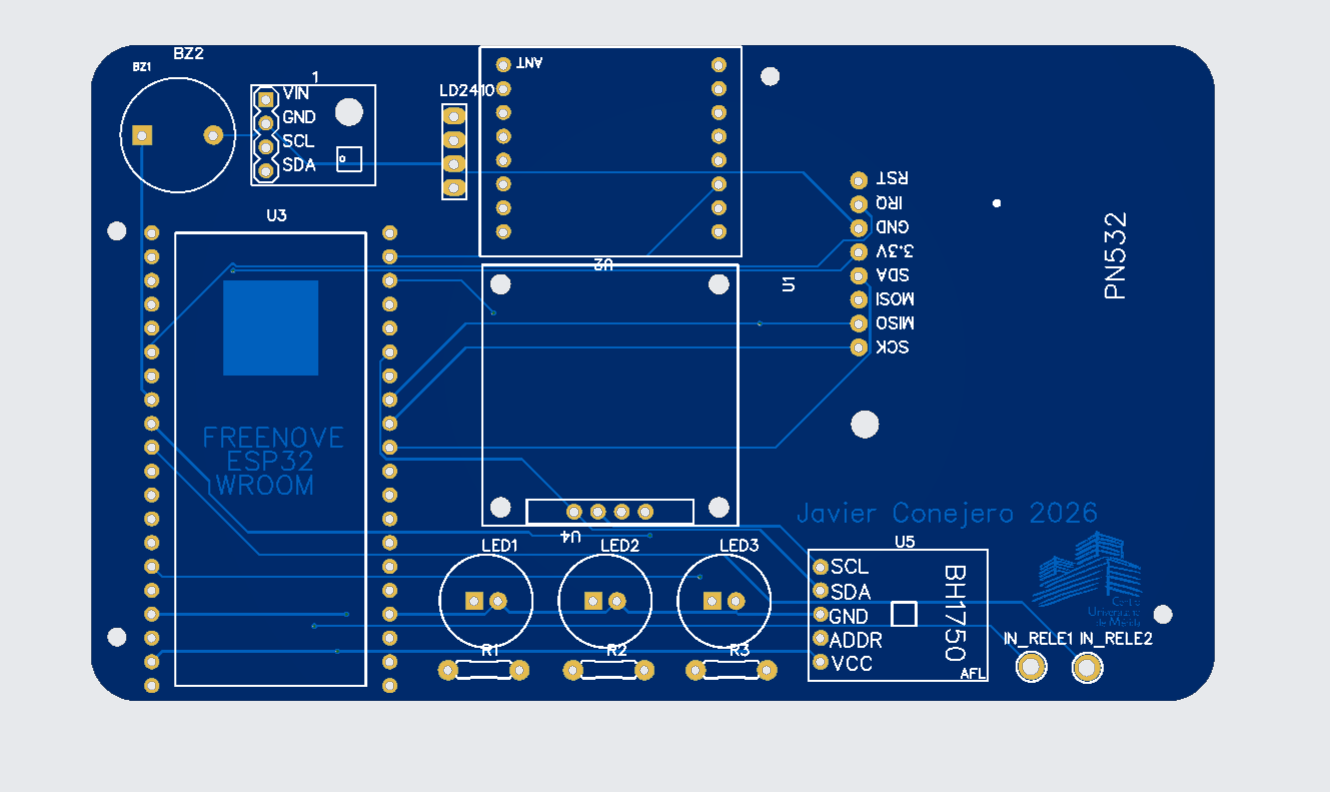
\includegraphics[width=0.9\textwidth]{imagenes/pcb.png}
\caption{\label{fig:pcb3} Resultado final del diseño de la PCB.}
\end{figure}

Esta placa convierte el prototipo en un dispositivo compacto y replicable, preparado para el despliegue de varios nodos.



\section{Monitor de red Cardputer M5}

Además de probar el sistema completo sobre hardware, con un nodo de aula con todos sus periféricos, el gateway y el servidor en una Raspberry Pi, la base de datos en otro equipo, se decide implementar un monitor de red para poder consultar el tráfico de la red LoRaLAN en tiempo real. Para ello, se implementó el monitor de red sobre un Cardputer M5 con el módulo SX1262. En la Figura~\ref{fig:cardputer1} se muestra un ejemplo de funcionamiento del monitor de red con un nodo conectado, donde se observan parámetros del nodo.


\begin{figure}[H]
\centering
        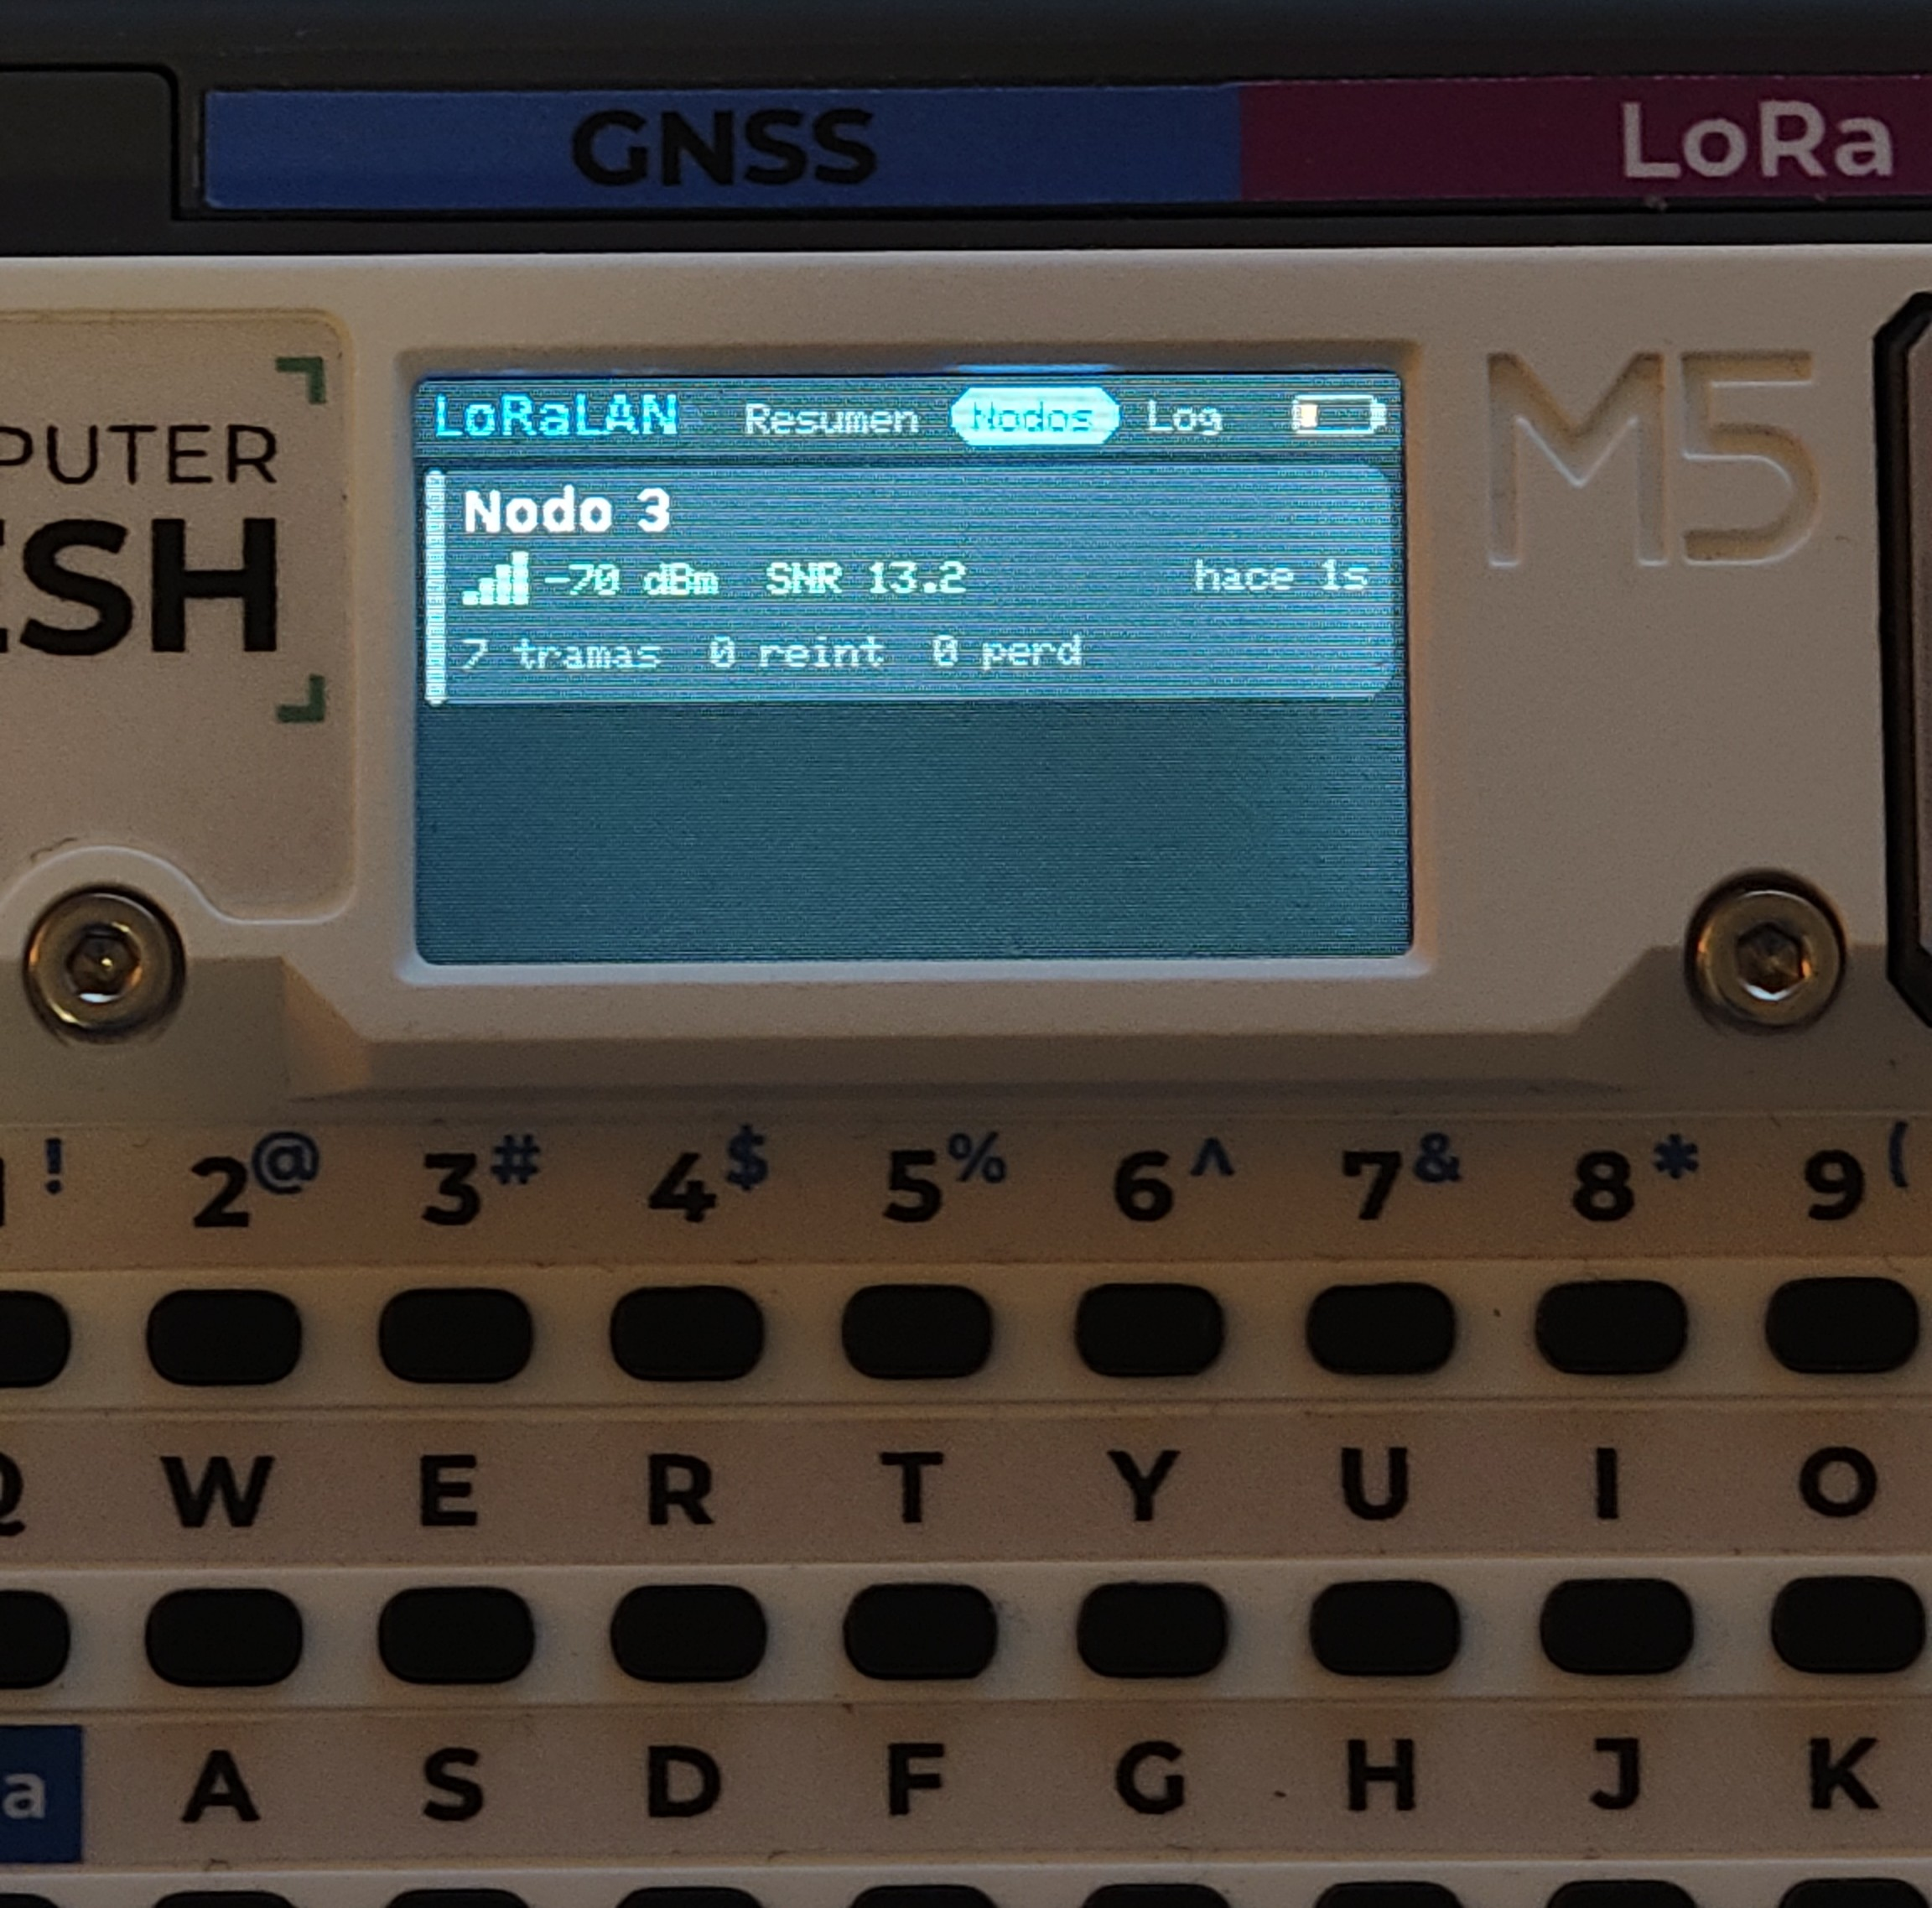
\includegraphics[width=0.8\textwidth]{imagenes/cardputer.jpg}
        \caption{Panel del monitor de red que muestra los nodos y algunos parámetros.}
        \label{fig:cardputer1}
\end{figure}

Se ha utilizado la placa LILYGO TTGO LoRa32 como hardware adicional para evaluar el comportamiento de la aplicación en hardware real. En este caso, se emplea la placa LILYGO con una versión modificada del firmware del nodo de aula, que funciona exactamente igual que el original, pero en lugar de poseer sensores y realizar lecturas sobre ellos, simula el envío de esta información. De esta manera se puede evaluar el funcionamiento del prototipo con dos nodos y un gateway y ver cómo se comporta la red con Cardputer.

\begin{figure}[H]
        \centering
        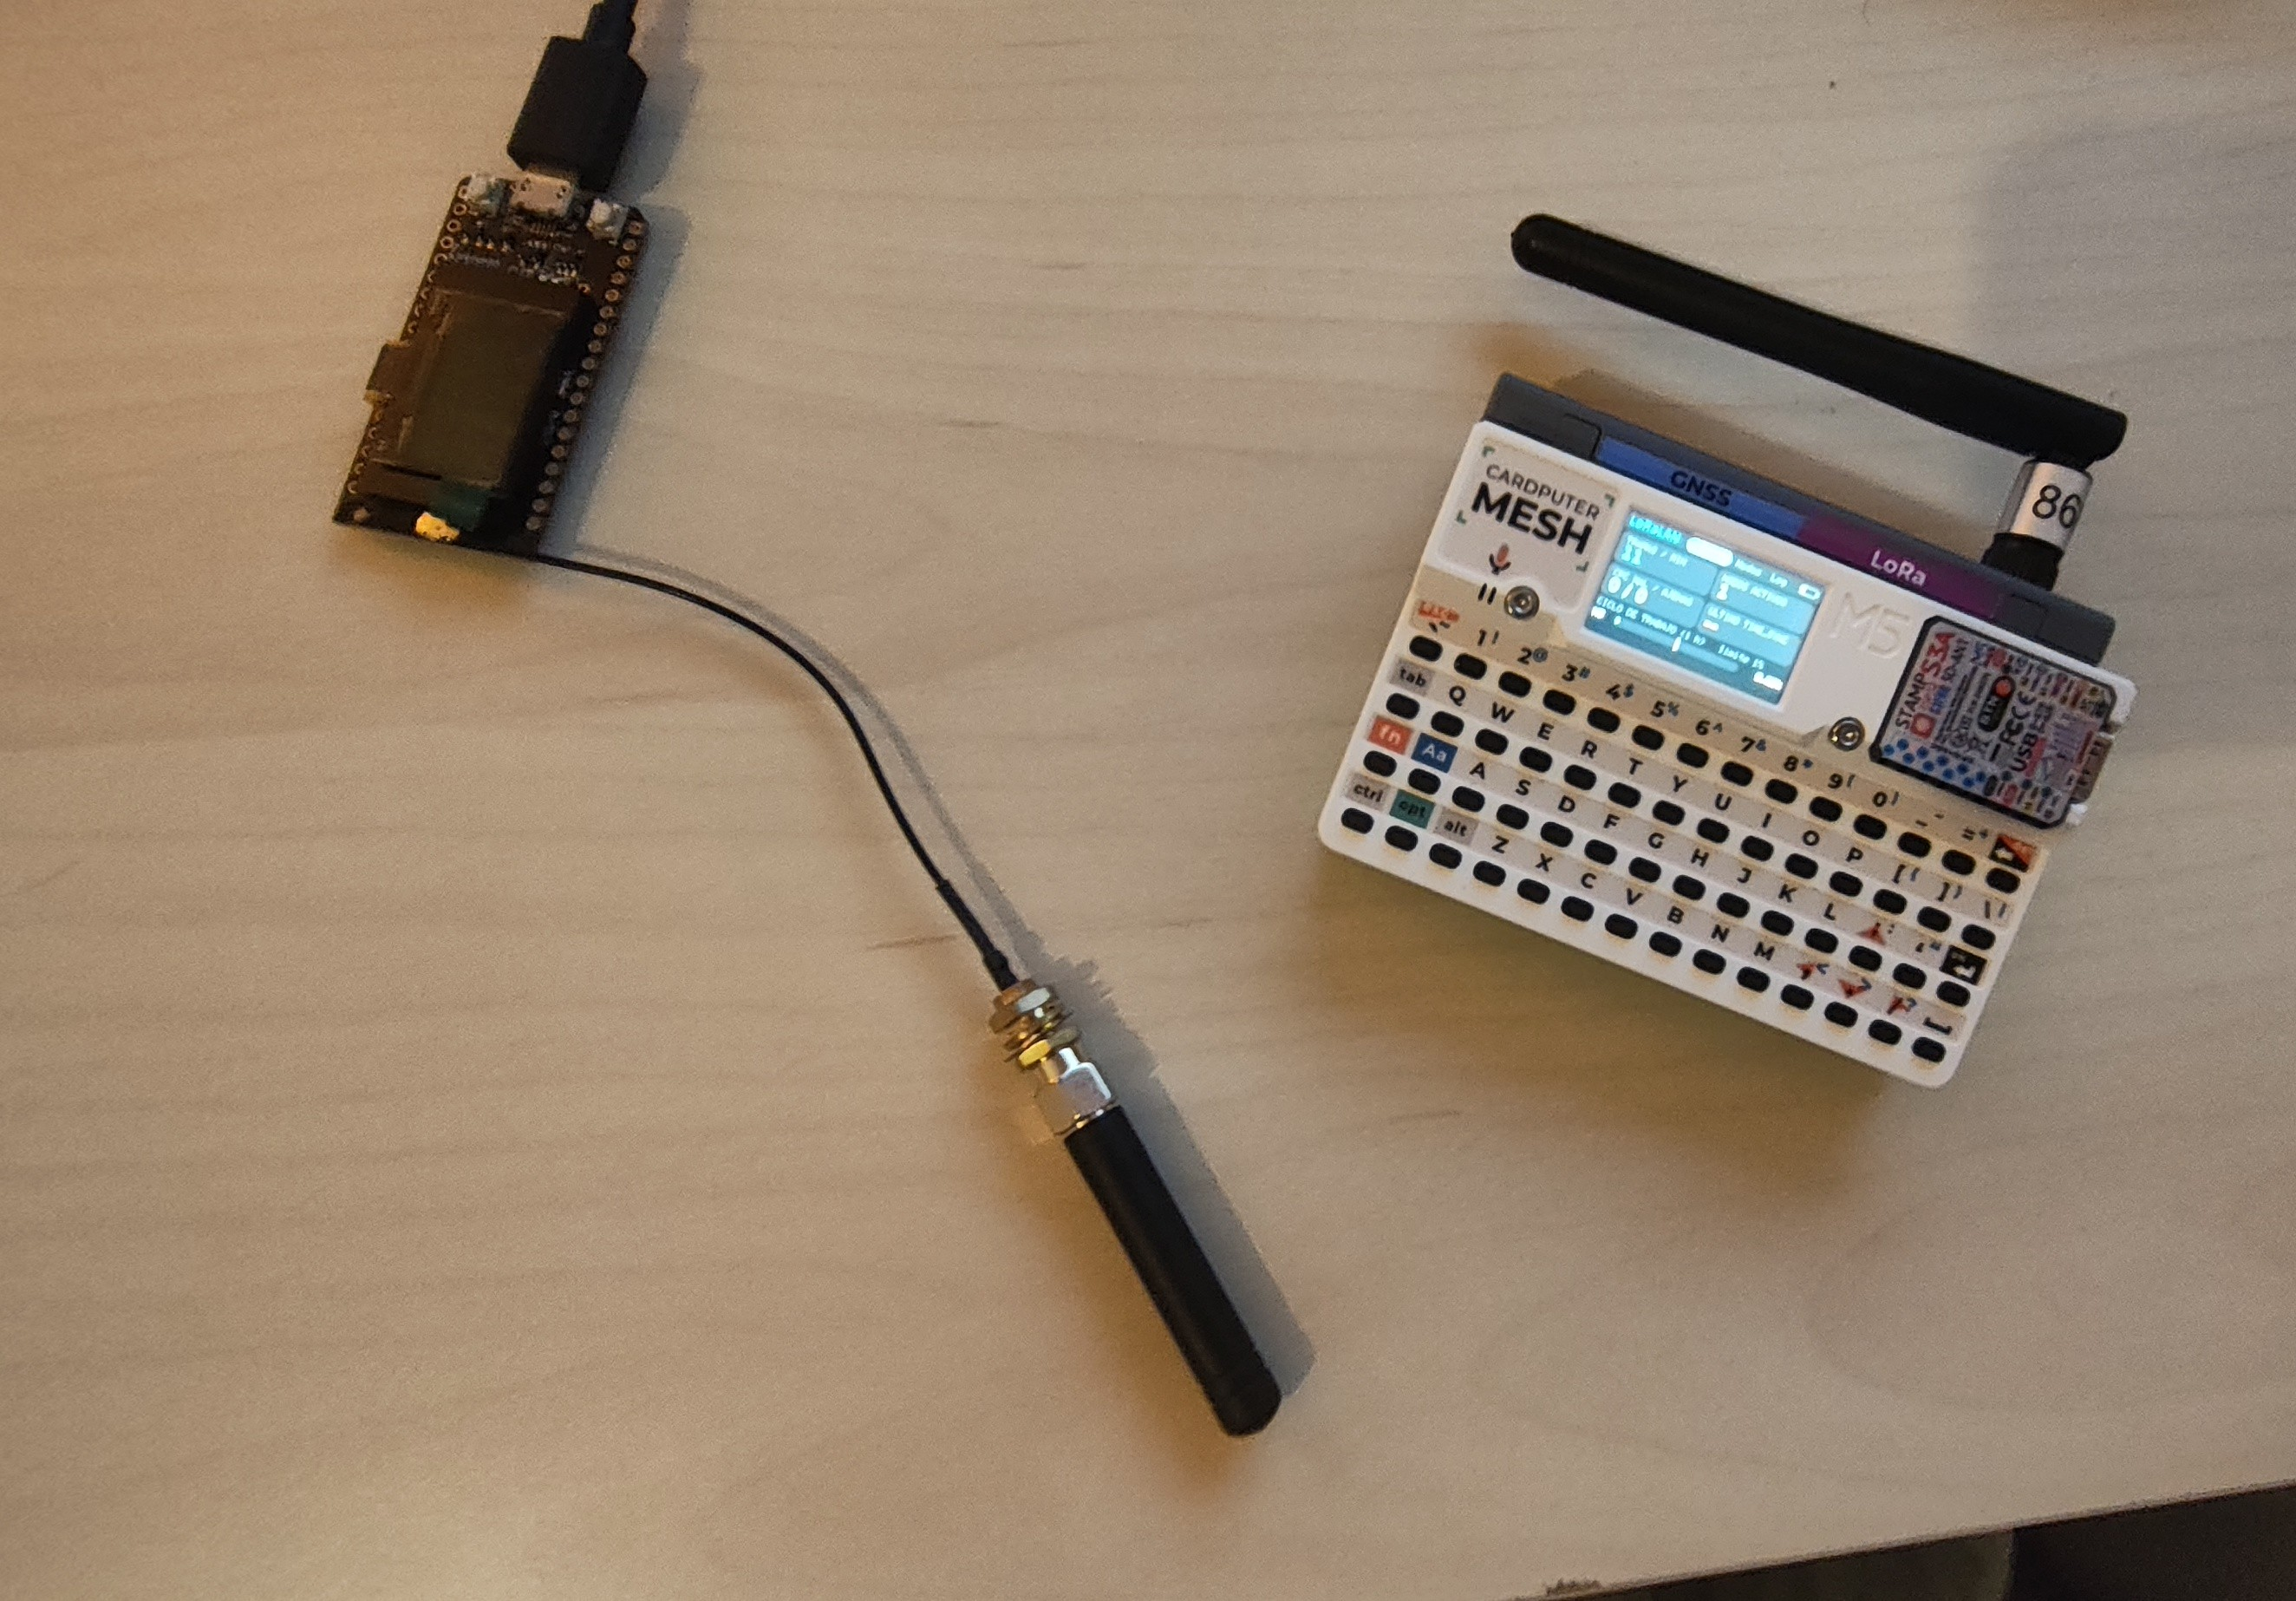
\includegraphics[width=1\textwidth]{imagenes/cardputer2.jpg}
        \caption{Monitor de red Cardputer y nodo simulado Lilygo.}
        \label{fig:imagen2}
\end{figure}





\section{Pruebas del sistema}

El sistema completo se ha probado además sobre hardware real, con un nodo de aula con todos sus periféricos, el gateway y el servidor en una Raspberry Pi, la base de datos en otro equipo y el monitor de red como observador independiente. Los escenarios ejercitados se muestran en la Tabla~\ref{tab:e2e}.

\begin{table}[H]
\centering
\small
\caption{\label{tab:e2e} Escenarios de la prueba de extremo a extremo.}
\begin{tabular}{|c|p{5.2cm}|p{7.8cm}|}
\hline
\textbf{N.º} & \textbf{Escenario} & \textbf{Resultado esperado} \\
\hline
1 & Arranque del nodo & Se asocia y el servidor lo da de alta. \\
\hline
2 & Tarjeta válida con clase & LED verde y nueva fila en la tabla de asistencias. \\
\hline
3 & Tarjeta desconocida & LED rojo y ningún registro. \\
\hline
4 & Fichaje con el servidor detenido & El nodo indica reintento y el fichaje se registra una sola vez al volver el servidor. \\
\hline
5 & Orden de relé desde el panel & El relé conmuta en pocos segundos y el panel refleja el nuevo estado. \\
\hline
6 & Supervisión & El panel muestra los sensores del aula. \\
\hline
7 & Reinicio de nodo & Desde el panel web por parte del administrador se envía la petición de reinicio a un nodo. \\
\hline
\end{tabular}
\end{table}

El sistema funcionó de extremo a extremo, de modo que los fichajes, la telemetría y las órdenes recorrieron la cadena completa.

